% TODO:
% - Add arritbutes cardinality hist after reduction
% - Add arttib distribution hists and compare with normla distribution - could compute mean , std, ..
% - Add anallysis of attrib correalation
% - Optionall - add some geographical/hisotrical conculstion about meteo Brenna data



\documentclass[10pt,a4paper]{article}

\usepackage{iftex} % <-- Add this to check the compiler

% Only load microtype if compiling with pdfLaTeX
\ifPDFTeX
  \usepackage[protrusion=true,expansion=true]{microtype}
\fi

\usepackage{fontspec}
\usepackage{polyglossia}
\usepackage{float}
\setmainlanguage{polish}
\setmainfont{Verdana} % Set Verdana as the main font

\usepackage{ragged2e}

\usepackage{graphicx} % No [pdftex] option here! XeLaTeX will auto-detect
\usepackage[
  colorlinks=true,
  linkcolor=black,
  urlcolor=black,
  citecolor=black,
  pdfborder={0 0 0}
]{hyperref} % Proper hyperref setup for xelatex

\usepackage{calc}
\usepackage{enumitem}

\frenchspacing
\linespread{1.15}

\usepackage[a4paper, lmargin=3.5cm, rmargin=2.5cm, tmargin=2.5cm, bmargin=2.5cm]{geometry}

\usepackage[all]{nowidow}

\usepackage{lipsum} % Dummy text

%-----------------------
% Set pdf information
%-----------------------
\hypersetup{ 	
  pdfsubject = {Example Subject},
  pdftitle = {Example Title},
  pdfauthor = {Your Name}
}
\graphicspath{{plots/}}
\graphicspath{{in/}}

%-----------------------
% Begin document
%-----------------------
\begin{document}
\begin{titlepage}
	\newgeometry{left=0cm, right=0cm, top=0cm, bottom=0cm}
    \centering
    \vspace*{5cm} % Adjust vertical space if needed

    {\Huge Raport Projektu EDA} \\[1.5cm]

    % Subtitle or any other text
    {\Large Feature engineering + EDA} \\[2cm]

    % Author
    {\large Bartłomiej Kózka} \\[0.5cm]

    % Date or any other info
    {\large \today} % You can replace \today with a custom date

    \vfill
	\restoregeometry 
\end{titlepage}


\justifying


\section{Wstęp}
Celem projektu jest wybranie odpowiedniego zestawu danych (nadającego się do wykorzystania w pipeline ML), a następnie wykonanie na nim inżynierii cech oraz eksploracyjnej analizy danych.
\subsection*{Dane}
Dane zostały wybrane z serwisu internetowego dane.gov.pl. Ilość danych znajdujących się na tej platformie jest duża, jednak większość tych danych nie nadawała by się do dalszej pracy w pipline ML. 
Na portalu dane.gov.pl można odnaleźć różne rodzaje danych w wielu kategoriach takich jak: edukacja, energia, gospodarka i finanse, transport i wiele innych. Dane można pobrać w formatach takich jak CSV, JSON, XML, Excel itp. Portal ten oferuje również łatwość w szybkim sprawdzeniu danych przez ich wizualizację (podgląd) na stronie portalu. Dane są również dostępne poprzez REST\_API. Dodatkowo można tam również znaleźć krótkie opisy badanych zestawów danych.
\subsection*{Wybór danych}
Nabyte dane pochodzą ze stacji meteorologicznej w Brennej z 2020 roku i zawierają zmienne takie jak: 
\textbf{\textit{date}} – data i godzina pomiaru, 
\textbf{\textit{ta}} (temperature) – temperatura powietrza wyrażona w stopniach Celsjusza, 
\textbf{\textit{rh}} (relative humidity) – wilgotność względna w procentach, 
\textbf{\textit{pr}} (pressure) – ciśnienie atmosferyczne w hektopaskalach, 
\textbf{\textit{wv}} (wind velocity) – średnia prędkość wiatru w metrach na sekundę (m/s), 
\textbf{\textit{wpmx}} (wind peak maximum) – maksymalna prędkość wiatru w metrach na sekundę, 
\textbf{\textit{wd}} (wind direction) – kierunek wiatru wyrażony w stopniach oraz 
\textbf{\textit{rf}} (rainfall) – wystąpienie opadów deszczu.
\begin{figure}[h]
	\centering
	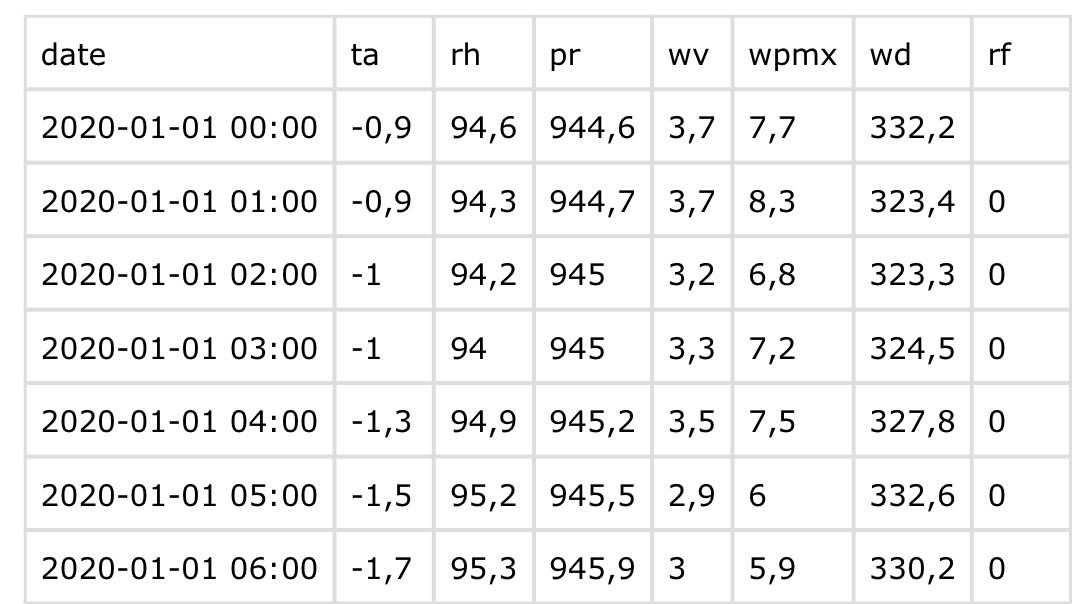
\includegraphics[scale=0.4]{Image.jpg}
	\caption{Dane meteorologiczne z Brennej}
	\label{fig:my_label}
\end{figure}

\newpage
\section{Pierwsze Etapy Pipeline'u ML}
Wstępna analiza danych polega na zrozumieniu struktury i charakterystyki zbioru danych. W tym kroku przeanalizowano podstawowe informacje o zbiorze, takie jak liczba próbek, liczba cech oraz typy danych. Zbadano również rozkład wartości w poszczególnych kolumnach oraz zidentyfikowano potencjalne problemy, takie jak brakujące wartości czy wartości odstające.

\vspace{1.5em} 

\subsection{Inżynieria cech (FE), Eskploracja danych (EDA)}
\vspace{1.5em} 
\subsection*{Wstępna analiza oraz cel wykorzystania danych}
Dane meteorologiczne mogą być wykorzystane w uczeniu maszynowym do różnych celów, takich jak: prognozowanie warunków pogodowych, klasyfikacja zdarzeń pogodowych, czy też dokładana predykcja wartości ciągłych, np. temperatury lub ilości opadów w mm. W tych przypadkach będziemy mówić o uczeniu nadzorowanym, ponieważ proces ten polega na wykorzystaniu danych wejściowych oraz odpowiednich etykiet, które model ma za zadanie przewidzieć.
\par
\hspace{0.75cm}
Pozyskane dane meteorologiczne z Brennej zawierają 8784 próbek (tyle co liczba godzin w roku przestępnym (366 dni) - 2020 - rok przestępny) oraz 8 cech. Wartości w kolumnach są typu zmiennoprzecinkowego, z wyjątkiem kolumny date, która jest typu datetime64[ns]. Pozostałe zmienne są ciągłe i wyrażają różne parametry meteorologiczne.
\par
\hspace{0.75cm}
Uwzględniając położenie stacji meteorologicznej w Brennej, która to jest częścią Beskidu śląskiego, z której pochodzą dane, mamy do czynienia z pogodą górską, która to charakteryzuje się duża zmiennością pogody. To znaczy, że warunki atmosferyczne mogą się znacznie różnić od tych w innych regionach Polski. W związku z tym, dane te mogą być szczególnie interesujące dla osób zajmujących się prognozowaniem pogody górskiej, badaniami klimatycznymi czy też dla turystów i mieszkańców regionu.
\begin{figure}[h]
	\centering
	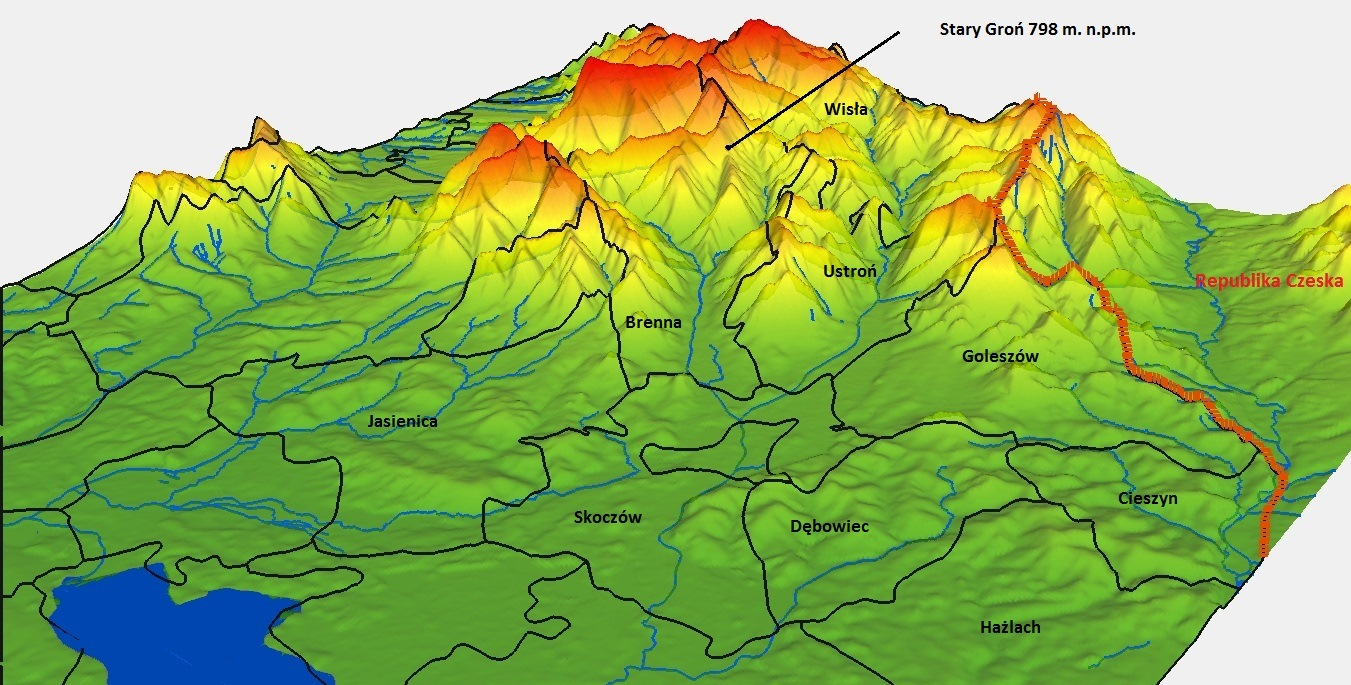
\includegraphics[scale=0.4]{plots/brenna-lokalizacja.jpg}
	\caption{Brenna - lokalizacja}
	\label{fig:my_label}
\end{figure}

\subsection*{Statystyki opisowe}
Dla każdej ze zmiennych obliczono cztery podstawowe miary statystyczne: wartość minimalną, średnią, odchylenie standardowe oraz wartość maksymalną.
\begin{figure}[H]
	\centering
	\includegraphics[scale=0.5]{plots/st_opis.png}
	\caption{Statystyki opisowe dla danych meteorologicznych}
	\label{fig:my_label}
\end{figure}
Zauważyć można, że temperatura powietrza (ta) osiąga wartości maksymalne powyżej 26°C, natomiast średnia pozostaje w granicach 7°C, co może być wynikiem znacznych wahań temperatury dobowej i sezonowej, typowych dla rejonów górskich. Wilgotność względna (rh) wykazuje dużą zmienność – przy średniej około 80% maksymalne wartości sięgają blisko 100%, co potwierdza wysoką wilgotność charakterystyczną dla terenów zalesionych i górskich. Ciśnienie atmosferyczne (pr), oscylujące wokół 930–970 hPa, wskazuje na dynamiczne warunki baryczne, często spotykane na obszarach o zróżnicowanej orografii.
\par
\hspace{0.75cm}
Prędkość wiatru (wv) i maksymalna prędkość porywu (wpmx), która osiąga blisko 30 m/s to jest ponad 100 km/h sugerują występowanie silniejszych zjawisk wiatrowych, co znajduje uzasadnienie w lokalizacji stacji – doliny i przełęcze sprzyjają przyspieszaniu mas powietrza. Kierunek wiatru (wd) wykazuje dużą rozpiętość wartości, co również jest typowe dla gór, gdzie kierunek wiatru bywa modyfikowany przez ukształtowanie terenu. Zmienna opadów (rf) cechuje się niską średnią, lecz wysoką wartością maksymalną, co potwierdza występowanie intensywnych, epizodycznych opadów – częstych w warunkach górskich, szczególnie w okresie letnim.
\par
\hspace{0.75cm}
Podsumowując, przedstawione dane dostarczają cennych informacji na temat lokalnych warunków klimatycznych w Beskidzie Śląskim. Ich analiza jak już wcześniej zostało wspomniane może służyć jako podstawa do dalszych badań nad mikroklimatem górskim.

\subsection*{Rozkłady cech}
\begin{figure}[H]
	\centering
	\includegraphics[scale=0.37]{plots/rozklad.png}
	\caption{Rozkład cech danych meteorologicznych}
	\label{fig:my_label}
\end{figure}
Spośród wszystkich analizowanych zmiennych szczególnie ciekawy rozkład wykazuje zmienna wd, odpowiadająca za kierunek wiatru. Zamiast jednolitego lub przypadkowego rozkładu, widoczne są wyraźne piki w kilku konkretnych kierunkach, co sugeruje, że w Brennej wiatry najczęściej wieją z określonych stron świata. Taki układ może odzwierciedlać lokalne uwarunkowania geograficzne, np. obecność dolin, grzbietów górskich czy wpływ dominujących mas powietrza, tak jak powyżej było to już wspomniane.

\subsection*{Wartości brakujące}

\begin{figure}[H]
	\centering
	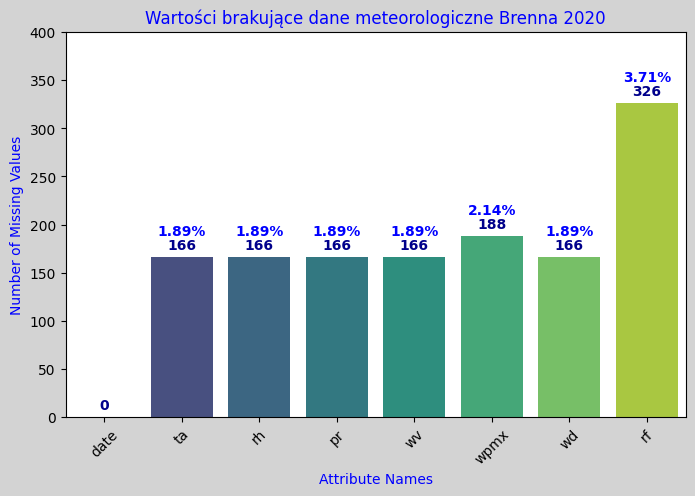
\includegraphics[scale=0.7]{missing_values.png}
	\caption{Wartości brakujące w danych meteorologicznych}
	\label{fig:my_label}
\end{figure}

Jak można zaobserwować na powyższym histogramie, tylko w kolumnie oznaczającej datę i godzinę pomiaru (date) nie występują żadne wartości brakujące co jest zgodne z oczekiwaniami, ponieważ jest to zmienna czasowa, która powinna być kompletna. Pozostałe zmienne zawierają pewną liczbę brakujących wartości.
W przypadku zmiennych takich jak temperatura (ta), wilgotność (rh), ciśnienie (pr), prędkość wiatru (wv), maksymalna prędkość wiatru (wpmx), kierunek wiatru (wd), liczba brakujących danych wynosi 166, co stanowi niewielki procent w porównaniu do całkowitej liczby próbek. Dla zmiennej rf (opady) brakujących wartości jest 326, co również jest małym procentem w odniesieniu do całkowitej liczby danych. W związku z tym, brakujące dane są stosunkowo niewielkie i nie mają istotnego wpływu na całościową strukturę danych.

\par
\hspace{0.75cm}
Biorąc pod uwagę niewielki procent brakujących danych oraz fakt, że braki są rozłożone równomiernie, można przyjąć, że brakujące wartości w danych meteorologicznych mają charakter \textbf{Missing Completely at Random (MCAR)}. Oznacza to, że brakujące dane są losowe i nie zależą od innych zmiennych w zbiorze danych. Prawdopodobnie przyczyną braków odczytów były zakłócenia w pracy czujników lub inne techniczne problemy związane z urządzeniami pomiarowymi.
\par
\hspace{0.75cm}
W celu przygotowania danych meteorologicznych do modelowania zastosowano dwie różne metody uzupełniania brakujących wartości, odpowiednio do charakteru poszczególnych zmiennych. Dla zmiennych ciągłych takich jak temperatura powietrza (ta), wilgotność względna (rh), ciśnienie atmosferyczne (pr), prędkość wiatru (wv), maksymalna prędkość porywu wiatru (wpmx) oraz kierunek wiatru (wd) zdecydowano się na interpolację liniową w funkcji czasu. Metoda ta pozwala na płynne oszacowanie brakujących wartości na podstawie danych sąsiednich, co odzwierciedla naturalne zmiany tych parametrów w czasie i zapewnia spójność czasową pomiarów.
\par
\hspace{0.75cm}
W przypadku zmiennej dotyczącej opadów (rf) przyjęto inne podejście: brakujące wartości zostały zastąpione zerami, ponieważ brak danych może oznaczać brak opadów, co jest logicznie uzasadnione i nie wprowadza istotnych zniekształceń do analizy.

\vspace{1.5em} 
\subsection*{Kardynalność cech}
Została obliczona kardynalność cech, czyli liczba unikalnych wartości dla każdej z cech. 
Na poniższym wykresie celowo kardynalość cechy date została pominięta, ponieważ jest to zmienna czasowa, która z definicji ma unikalne wartości dla każdej godziny w roku. Pozostałe zmienne mają różną kardynalność, co może wpływać na dalszą analizę i modelowanie. Wartości kardynalności dla poszczególnych zmiennych przedstawione są na poniższym wykresie.

\begin{figure}[h]
	\centering
	\includegraphics[scale=0.7]{plots/car_before.png}
	\caption{Kardynalność cech przed redukcją}
	\label{fig:my_label}
\end{figure}
\noindent W przedstawionych wynikach liczby unikalnych etykiet zmiennych, zauważalna jest szczególnie wysoka kardynalność w przypadku zmiennej wd (kierunek wiatru), która liczy aż 3022 unikalnych wartości. Taki wynik jest wynikiem precyzyjnego pomiaru w stopniach, co skutkuje dużą liczbą unikalnych kategorii. Pozostałe zmienne, takie jak temperatura (ta), wilgotność (rh), ciśnienie (pr), prędkość wiatru (wv), maksymalna prędkość porywu wiatru (wpmx) oraz opady (rf), wykazują raczej umiarkowaną liczbę unikalnych wartości, co jest typowe dla danych meteorologicznych i nie stanowi problemu w dalszej analizie.
\par
\hspace{0.75cm}
W celu uproszczenia analizy danych meteorologicznych, zdecydowano się na redukcję zmiennej wd (kierunek wiatru). Z uwagi na fakt, iż jest to cecha, która nie wyamaga precyzji co do dziesiętnej części ułamka do predykcji jej samej (co i tak może być bradzo cieżkim wyzwaniem), jak i zarówno w kontekście bycia zmienną objaśnijącą dla innnej zmiennej objaśnianej, postanowiono zredukować jej precyzję na liczby całkowitę co będzie w zupełności wystarczalne w dalszej częsci pipline'u ML.
Można by również pomyśleć nad redukcją tej zmiennej do 8 kategorii (N, NE, E, SE, S, SW, W, NW), jednakże w tym przypadku nie jest to konieczne.
\par
\hspace{0.75cm}
Pozostałe zmienne, takie jak temperatura, wilgotność czy ciśnienie, pozostają w oryginalnej formie, ponieważ zawierają cenne informacje, które mogą wpływać na przewidywania związane z opadami i innymi zjawiskami meteorologicznymi.
\par
\hspace{0.75cm}
Wartościową operacją w kontekście dalszego przebiegu pipeline'u mogło by róweniż być zredukowanie cechy rf (rainfall) na zmienną binarną (0 lub 1), co oznaczało by brak opadów lub ich występowanie. Jednakże na tym etapie pipeline'u nie jest to wskazane, ze względów na brak wiedzy co do dalszego wykorzystania danych. W przypadku chęci predykcji jak duże są opady w zależnoći od innych zmiennych, sprowadzenie tej zmiennej do wartości binarnej było by kategorycznym błędem.
\begin{figure}[h]
	\centering
	\includegraphics[scale=0.7]{plots/st_after.png}
	\caption{Kardynalność cech po redukcji zmiennej wd}
	\label{fig:my_label}
\end{figure}


\vspace{1.5em} 
\subsection*{FE - Dodanie wartościowych zmiennych}
Po przeanalizowaniu oraz redukcji kardynalości cech, zdecydowano się na dodanie nowych zmiennych, które mogą być istotne w kontekście dalszej analizy i modelowania. Wprowadzono następujące zmienne:
\par
\hspace{0.75cm}
\textbf{season (pora roku)} – zmienna kategoryczna, która wskazuje na porę roku (wiosna, lato, jesień, zima). Zmienna ta została dodana w celu uwzględnienia sezonowości w danych meteorologicznych. W różnych porach roku warunki atmosferyczne mogą się znacznie różnić, co może mieć wpływ na występowanie opadów i inne zjawiska pogodowe.
\par
\hspace{0.75cm}
\textbf{wd\_cat (kierunek wiatru ze względu na kierunki geograficzne)} – zmienna kategoryczna, która wskazuje na kierunek wiatru w czterech głównych kierunkach geograficznych (N, E, S, W). Zmienna ta została dodana w celu uproszczenia analizy kierunku wiatru i umożliwienia lepszego zrozumienia jego wpływu na inne zmienne meteorologiczne, bez konieczności wchodzenia w szczegółowy (kątowy) opis kierunku waitru.
\par
\hspace{0.75cm}
\textbf{rf\_bin {opady deszczu (0 lub 1)}} – zmienna binarna, która wskazuje na wystąpienie opadów deszczu (1) lub ich brak (0). Zmienna ta została również dodana w celu uproszczenia analizy i umożliwienia lepszego zrozumienia wpływu innych zmiennych na występowanie opadów, np. w kontekśście przewidywania czy opady miały miejsce czy nie.
\begin{figure}[H]
	\centering
	\includegraphics[scale=0.7]{plots/car_after_add.png}
	\caption{Kardynalność cech po dodaniu nowych zmiennych}
	\label{fig:my_label}
\end{figure}




\vspace{1.5em} 
\subsection*{Wartości odstające}
\begin{figure}[H]
	\centering
	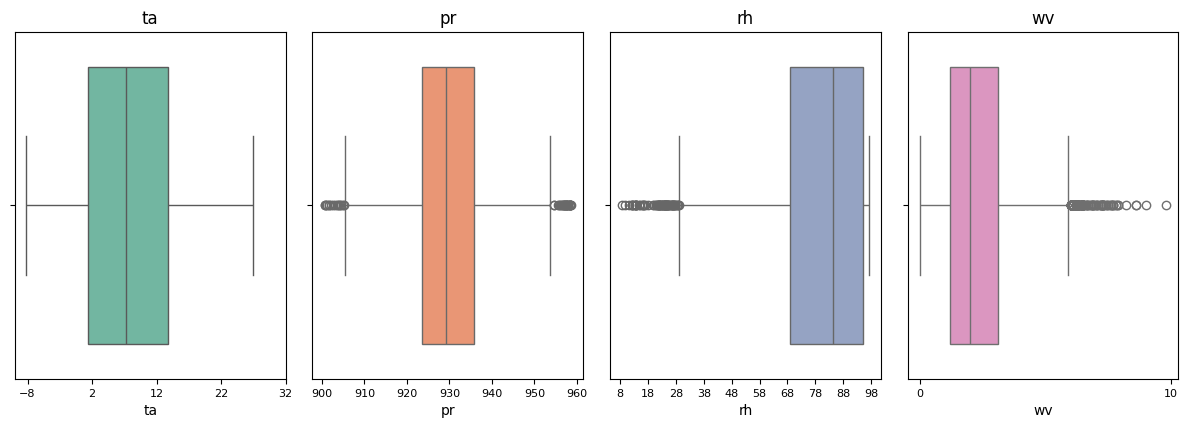
\includegraphics[scale=0.5]{boxplot.png}
	\caption{Wartości odstające}
	\label{fig:my_label}
\end{figure}
\noindent Po przeprowadzeniu analizy danych w celu odnalezniie anomalii nie wykryto obecności wyraźnych wartości odstających (outlierów) w zestawie danych meteorologicznych. Wszystkie zmienne rozkładają się w sposób typowy dla danych tego typu, a wartości skrajne, jeśli występują, nie odbiegają znacząco od ogólnych wzorców. W związku z tym, dane zostały uznane za stabilne i nie wymagały dalszej obróbki w zakresie usuwania wartości odstających.


\vspace{1.5em} 
\subsection*{Macierz korelacji}
\begin{figure}[H]
	\centering
	\includegraphics[scale=0.7]{plots/heatmap.png}
	\caption{Korelacja pomiędzy zmiennymi}
	\label{fig:my_label}
\end{figure}
Na podstawie analizy można zauważyć silną dodatnią korelację między średnią prędkością wiatru (wv) a jego maksymalną wartością (wpmx), osiągającą wartość 0,93. Wskazuje to na dużą współzmienność obu zmiennych – dni z wyższą średnią prędkością wiatru charakteryzują się również wyższym wiatrem maksymalnym. Umiarkowanie silna ujemna korelacja (r = -0,45) występuje między temperaturą powietrza (ta) a ciśnieniem atmosferycznym (pr), co może odzwierciedlać wpływ lokalnych warunków pogodowych oraz sezonowych układów ciśnienia. Zmienna sezonowa (season), wyodrębniona z daty, wykazuje dodatnią korelację zarówno z temperaturą (r = 0,50), jak i z samą datą (r = 0,57), co potwierdza wpływ pory roku na rozkład temperatury i chronologiczną strukturę danych.
Zmienna opadowa (rf) oraz jej wersja binarna (rf\_bin) również wykazują ze sobą silną zależność (r = 0,52), co jest spodziewane ze względu na logiczną konwersję wartości ciągłej na kategorię obecności lub braku opadu. Pozostałe korelacje między zmiennymi są słabe lub bardzo słabe, co sugeruje niewielkie liniowe zależności bądź możliwość występowania relacji nieliniowych, niewidocznych w analizie korelacji Pearsona.

\vspace{1.5em} 
\subsection{Uczenie nadzorowane}
\vspace{1.5em} 
\subsection*{Wybór zmiennej Target}
Jako zmienną TARGET wybrano \textbf{temperaturę powietrza (ta)}.
Temperatura jest jedną z kluczowych wielkości meteorologicznych — wpływa na życie ludzi, roślinność i cykle przyrody. Jest też najczęściej prognozowaną zmienną w meteorologii. W warunkach klimatu górskiego, gdzie występują duże dobowe i sezonowe wahania temperatury, jej przewidywanie jest szczególnie istotne, m.in. z powodu wpływu na lokalne zjawiska pogodowe, transport czy rolnictwo. Ukształtowanie terenu (np. doliny, stoki) dodatkowo wzmacnia lokalne różnice temperatur, co sprawia, że jest to naturalny wybór jako zmienna do modelowania.

\vspace{1.5em} 
\subsection*{Wybór zmiennych Features}
Wybrane zmienne FEATURES to:

\noindent \textbf{Ciśnienie (pr)} – zmiany ciśnienia wiążą się z przemieszczaniem mas powietrza i frontów atmosferycznych, które w rejonach górskich silnie wpływają na zmiany temperatury.

\noindent \textbf{Wilgotność (rh)} – powietrze w górach często ma zmienną wilgotność; duża wilgotność może ograniczać nagrzewanie, a suchy klimat sprzyja szybkiemu nagrzewaniu się powietrza.

\noindent \textbf{Wiatr (wv, wpmx)} – w terenie górskim wiatr pełni ważną rolę w przenoszeniu mas powietrza między wysokościami i dolinami, co bezpośrednio wpływa na temperaturę.

\noindent \textbf{Pora roku (season)} – sezon wpływa na długość dnia, nasłonecznienie oraz częstość występowania zjawisk takich jak inwersje temperatury, które są typowe dla dolin górskich.


\vspace{1.5em}
\par
\hspace{0.75cm}
Nie uwzględniono kierunku wiatru (wd) ani opadów (rf), ponieważ ich wpływ na temperaturę jest bardziej pośredni i trudniejszy do jednoznacznego ujęcia.

\vspace{5em} 
\subsection*{Źródła}
\begin{itemize}
	\item \url{https://brenna.meteo.com.pl/}
\end{itemize}


\end{document}
